\documentclass[11pt]{article}
\usepackage{graphicx}
\usepackage{listings}
\usepackage{anysize}
\renewcommand{\topfraction}{0.9}    % max fraction of floats at top
\renewcommand{\bottomfraction}{0.8}
\marginsize{2cm}{2cm}{1cm}{2cm}
\lstset{
  language=C,                     % choose the language of the code
}
\begin{document}

\title{Algorithms Coursework}
\author{Xueqi Chen and Haixiao Su}

\maketitle
\section*{Randomised Algorithms}
The below figures indicates the changes in time/number of executions in proportional to the size of the words added into the set for three different randomised algorithms: Skip List, Bloom Filter and Randomised BST. The observed trend for time complexity for Skip List and Bloom Filter all follows the similar pattern, which is predicted to be O(log n).
\section*{Add}
\begin{figure}[ht]
\centering
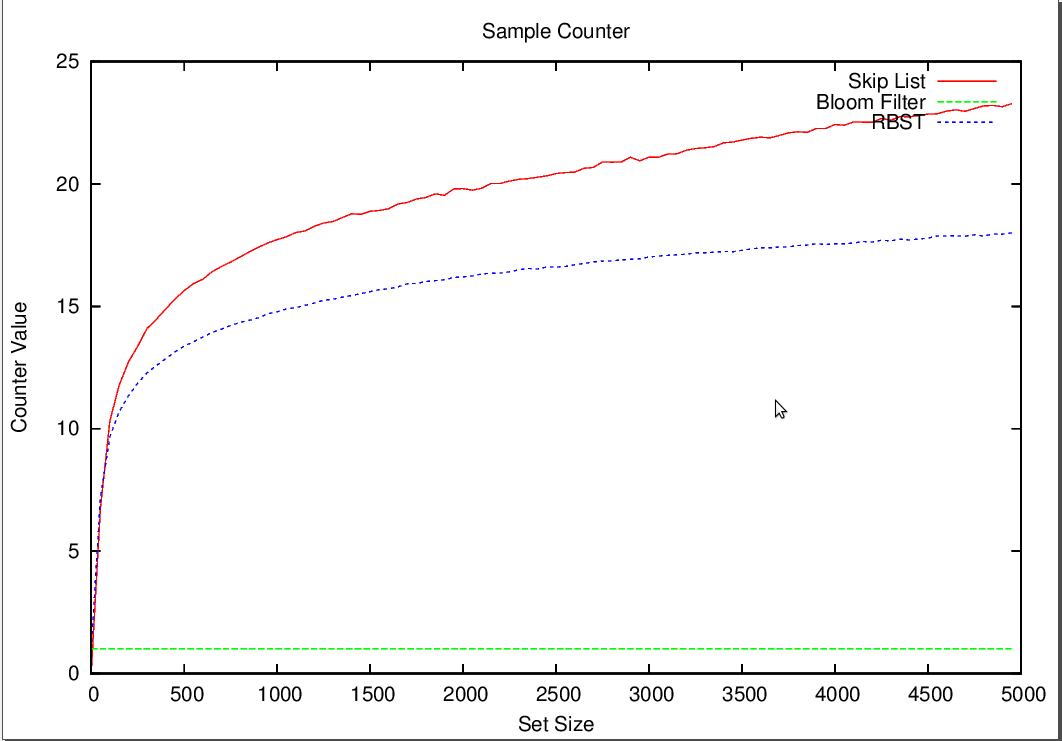
\includegraphics[height=70mm,width=100mm]{addcounter.png}
\caption{addcounter}
\end{figure}
\begin{figure}[ht]
\centering
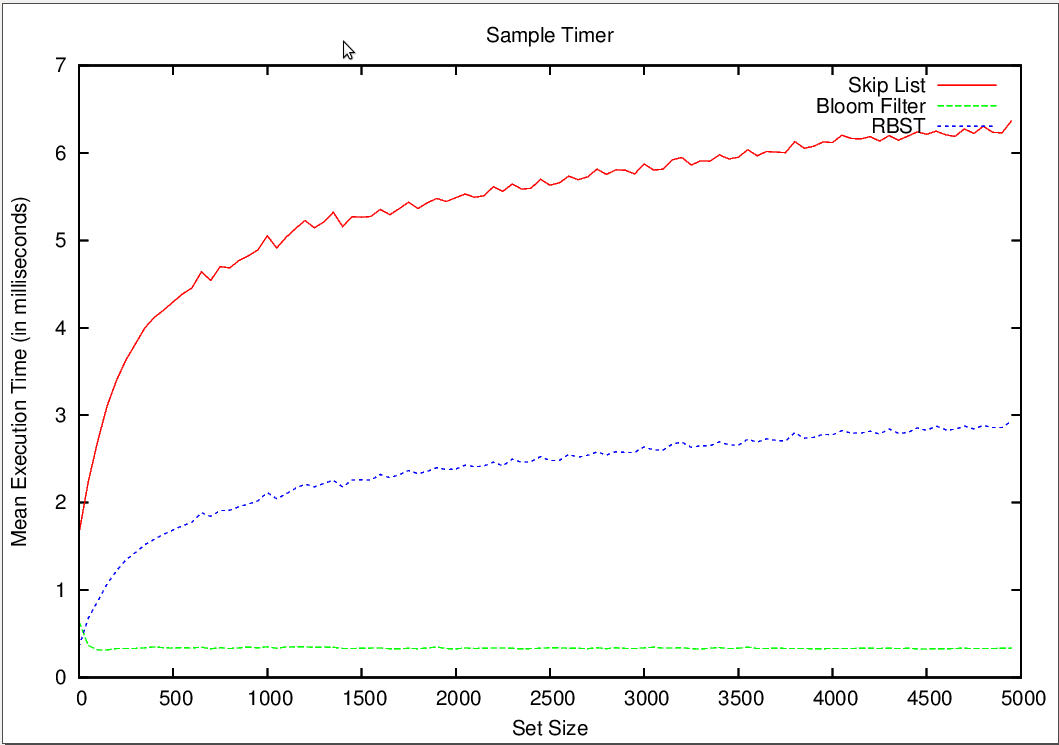
\includegraphics[height=70mm,width=100mm]{addtimer.png}
\caption{addtimer}
\end{figure}
\subsection*{Skip List}
Skip List add function uses randomization
generate new j-link element then search to find a position for the new element
and link it in as we move down to each level. The time complexity as shown in figure 2, is proportional to the size of the skip list and is bounded by the height of the skip list so thus O(log n). In other words, as there is more words added into the list, the time it takes to add each word becomes relatively less.

\section{Delete}
\begin{figure}[ht]
\centering
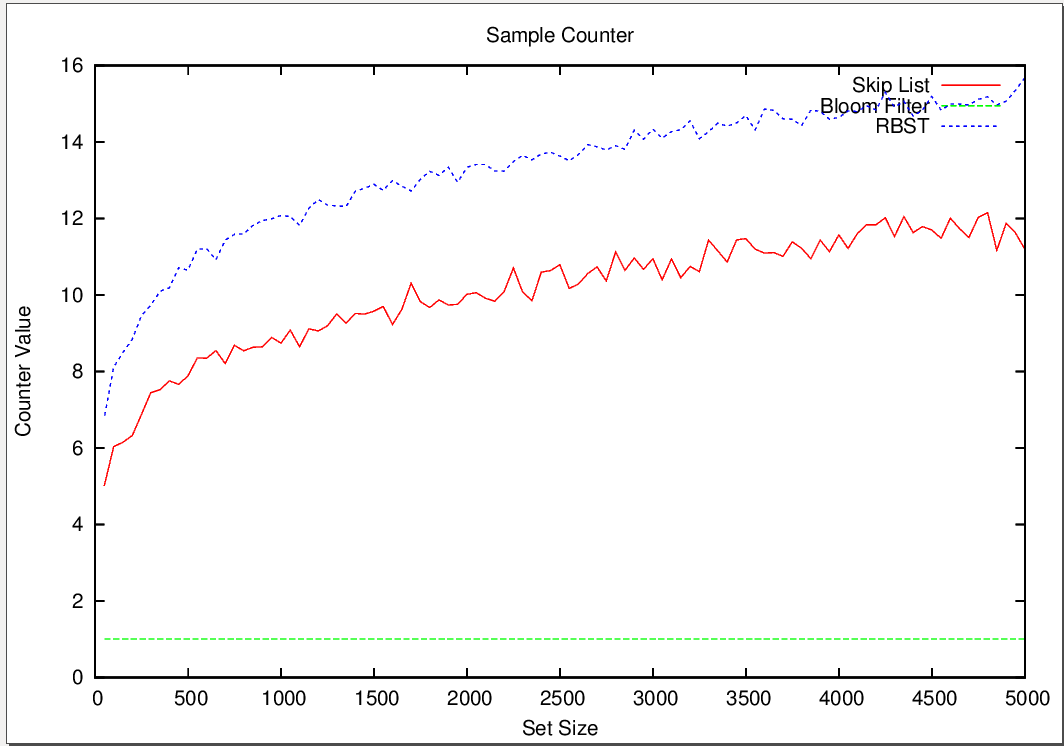
\includegraphics[height=70mm,width=100mm]{delcounter.png}
\caption{delcounter}
\end{figure}
\begin{figure}[ht]
\centering
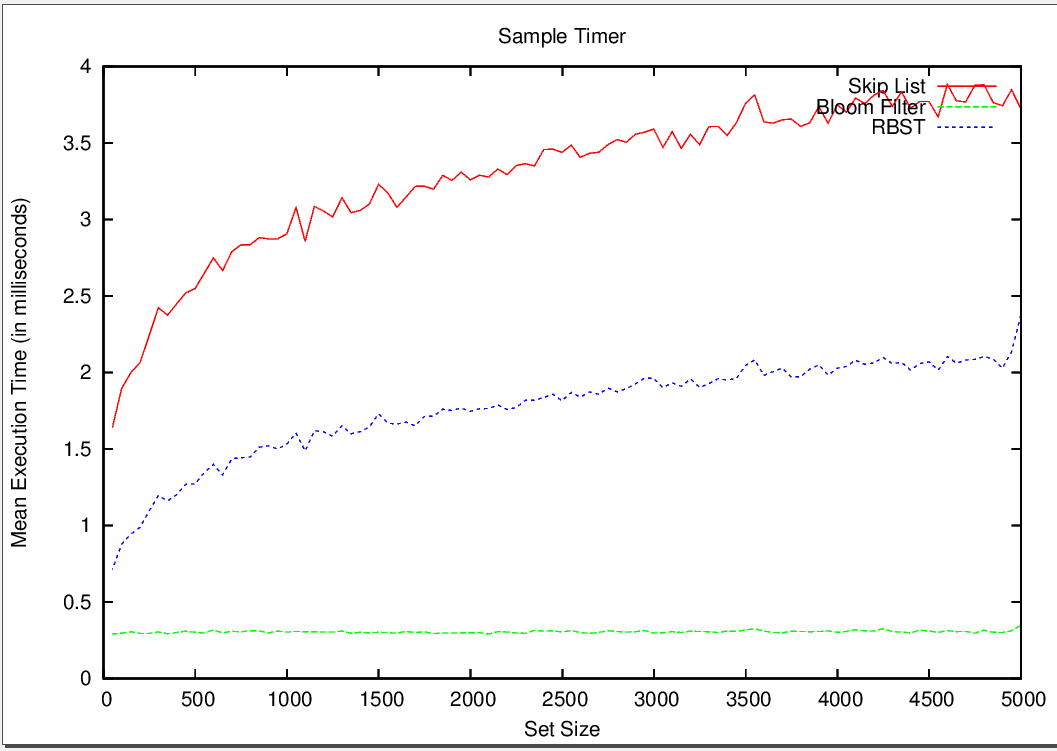
\includegraphics[height=70mm,width=100mm]{deltimer.png}
\caption{deltimer}
\end{figure}



\section{Find}
\begin{figure}[ht]
\centering
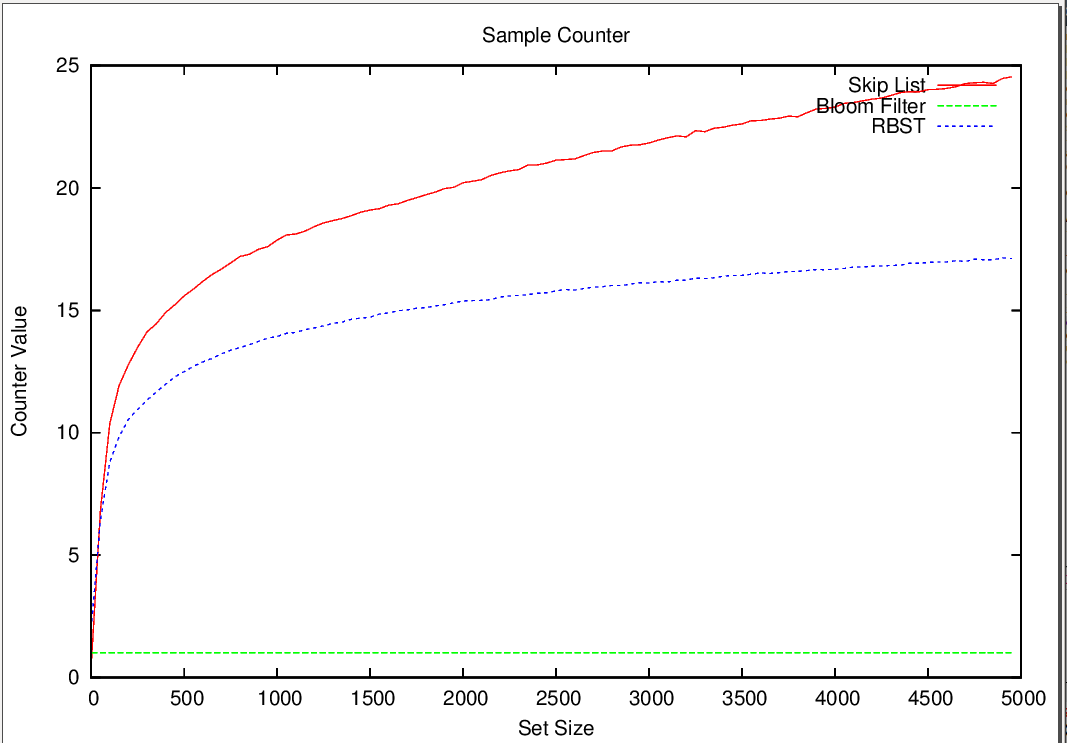
\includegraphics[height=70mm,width=100mm]{findcounter.png}
\caption{findcounter}
\end{figure}
\begin{figure}[ht]
\centering
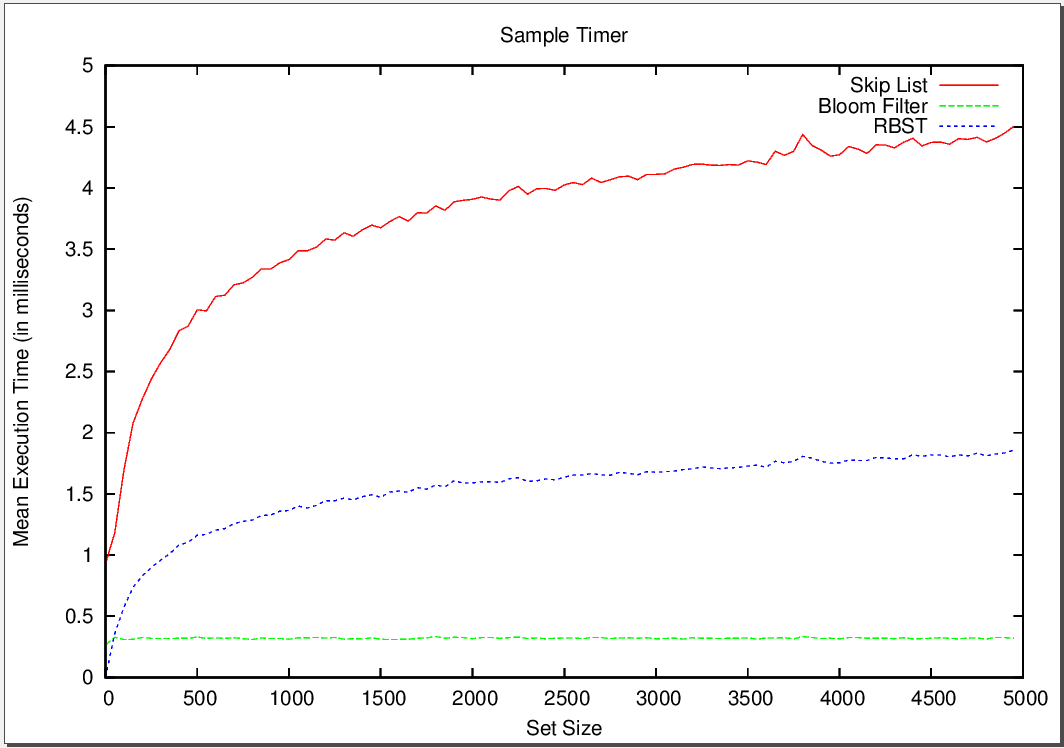
\includegraphics[height=70mm,width=100mm]{findtimer.png}
\caption{findtimer}
\end{figure}


\end{document}